
\subsection{Cohesive Elements}

The cohesive elements that have been implemented in \akantu are based
on the work of Ortiz and Pandolfi~\cite{ortiz1999}. Their main
properties are reported in Table~\ref{tab:coh:cohesive_elements}.

\begin{table}[!htb]
\begin{center}
\begin{tabular}{l|llcc}
\toprule
Element type & Facet type & Order & \# nodes & \# quad. points  \\
\midrule
\texttt{\_cohesive\_1d\_2} & \texttt{\_point\_1} & linear & 2 & 1  \\
\hline
\texttt{\_cohesive\_2d\_4} & \texttt{\_segment\_2} & linear & 4 & 1  \\
\texttt{\_cohesive\_2d\_6} & \texttt{\_segment\_3} & quadratic & 6 & 2  \\
\hline
\texttt{\_cohesive\_3d\_6} & \texttt{\_triangle\_3} & linear & 6 & 1  \\
\texttt{\_cohesive\_3d\_12} & \texttt{\_triangle\_6} & quadratic & 12 & 3  \\
\bottomrule
\end{tabular}
\end{center}
\caption{Some basic properties of the cohesive elements in \akantu.}
\label{tab:coh:cohesive_elements}
\end{table}

\begin{figure}
  \centering
  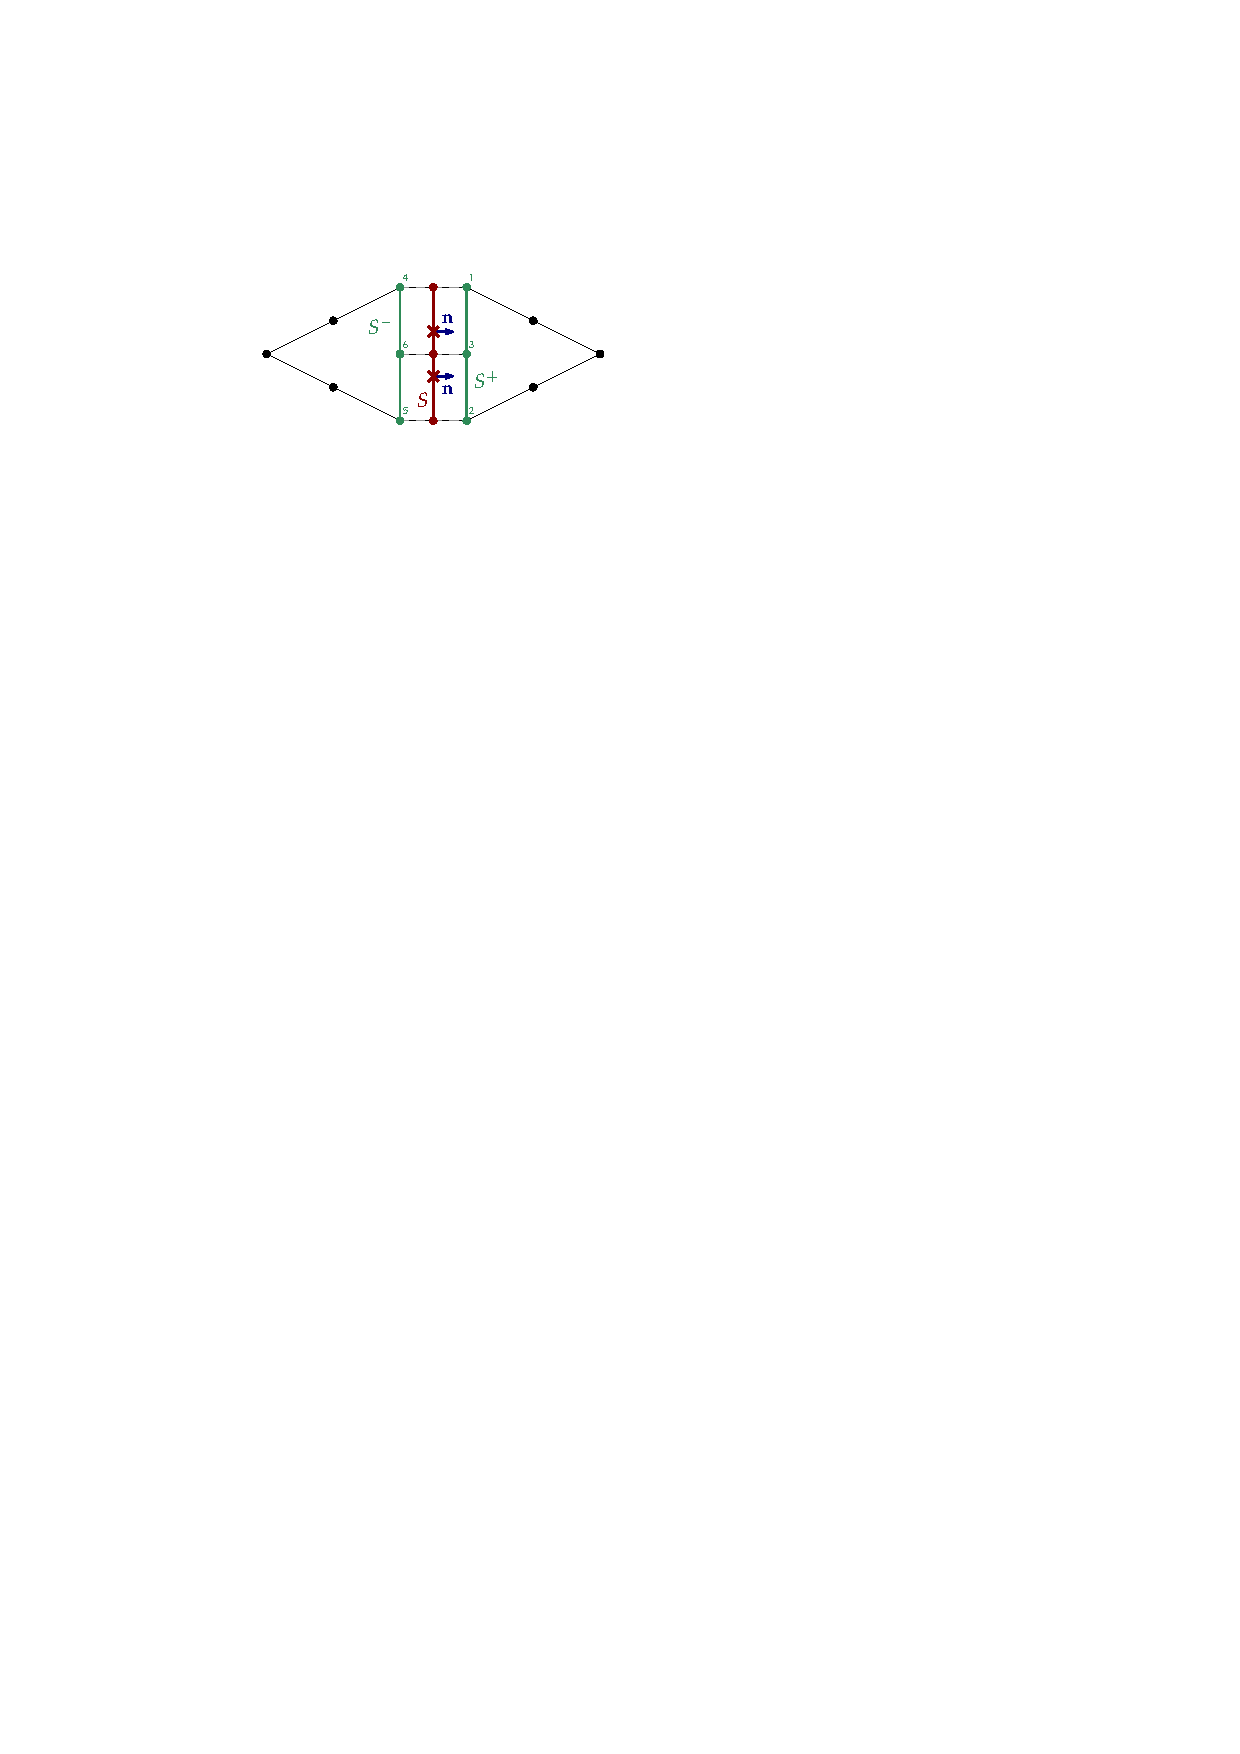
\includegraphics[width=.6\textwidth]{figures/cohesive2d}
  \caption{Cohesive element in 2D for quadratic triangular elements
    T6.}
  \label{fig:smm:coh:cohesive2d}
\end{figure}

Cohesive element insertion can be either realized at the beginning of
the simulation or it can be carried out dynamically during the
simulation. The first approach is called \emph{intrinsic}, the second
one \emph{extrinsic}. When an element is present from the beginning, a
bilinear or exponential cohesive law should be used instead of a
linear one. A bilinear law works exactly like a linear one except for
an additional parameter $\delta_0$ separating an initial linear
elastic part from the linear irreversible one. For additional details
concerning cohesive laws see Section~\ref{sec:cohesive-laws}.

\begin{figure}
  \centering
  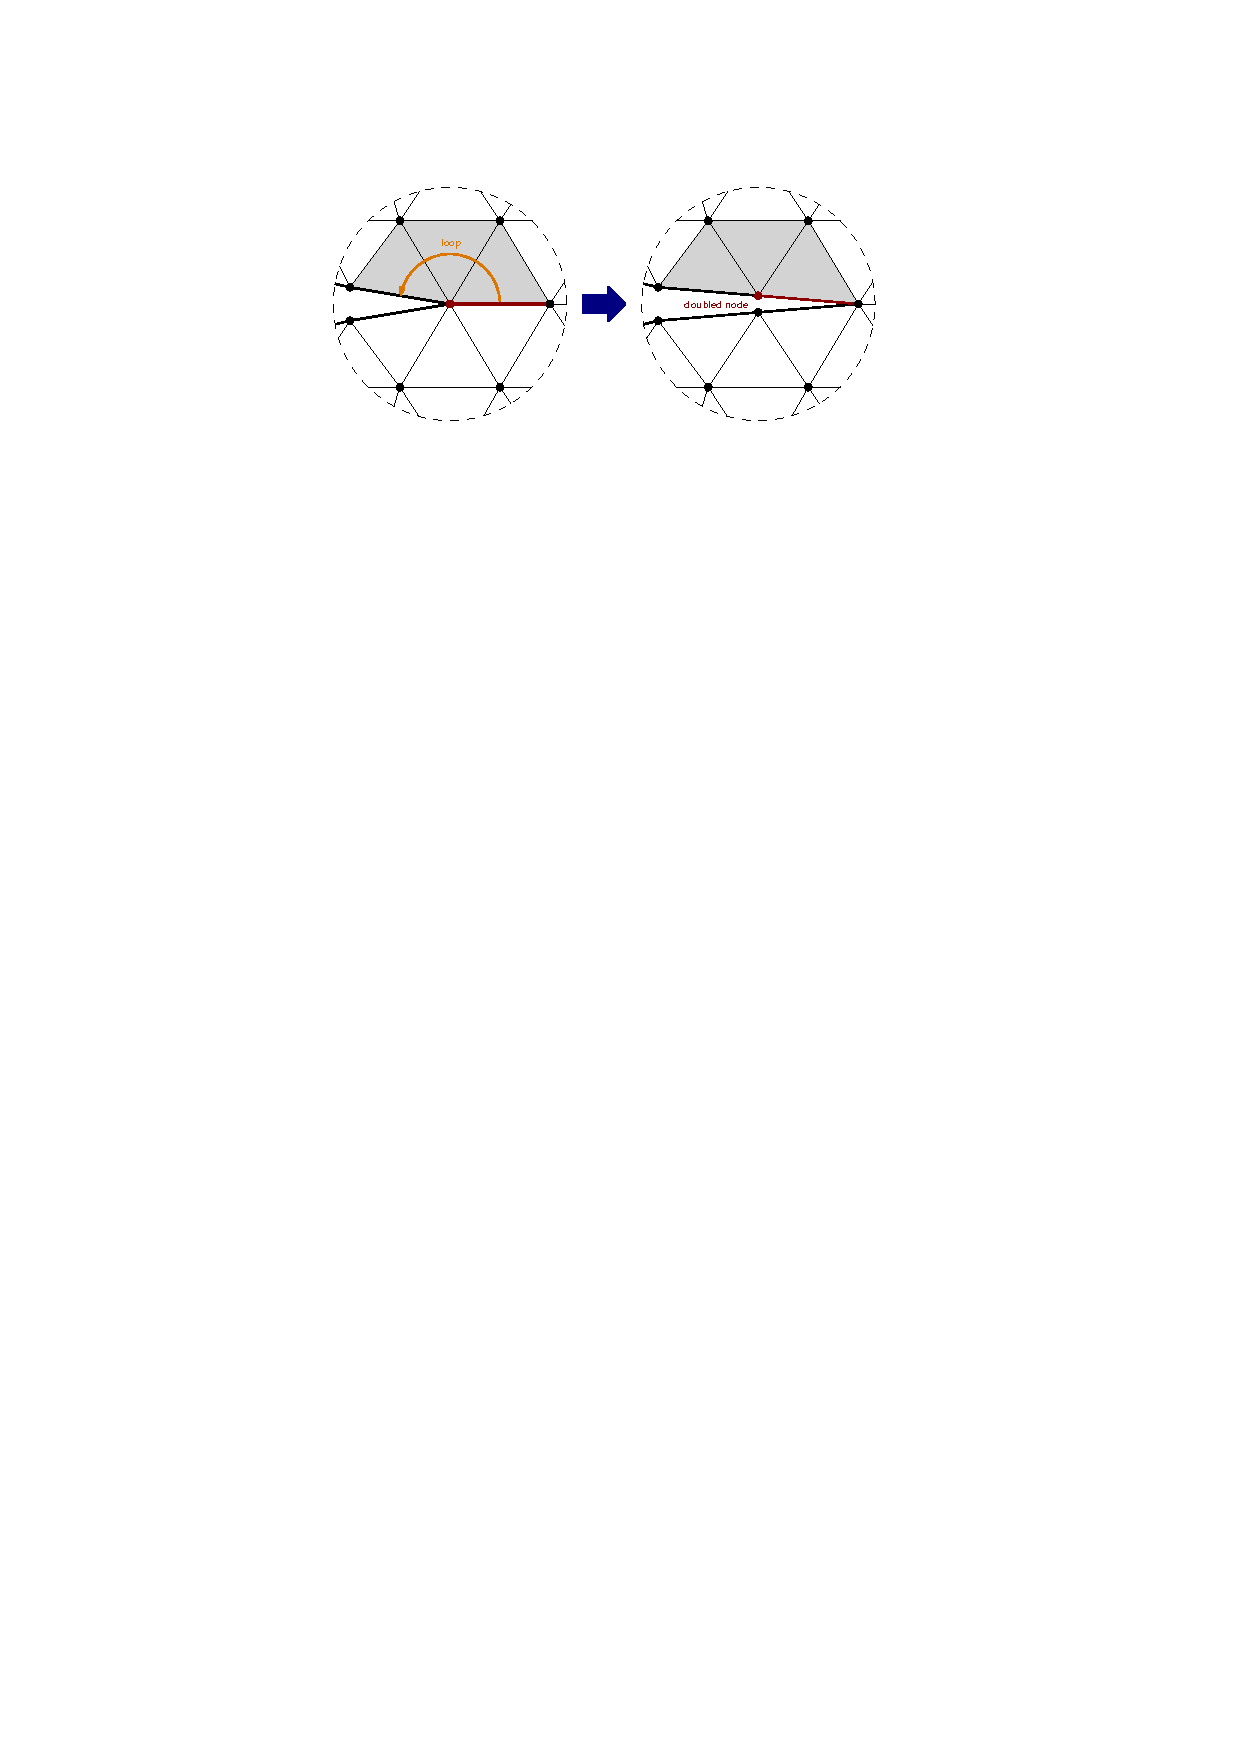
\includegraphics[width=.75\textwidth]{figures/insertion}
  \caption{Insertion of a cohesive element.}
  \label{fig:smm:coh:insertion}
\end{figure}

Extrinsic cohesive elements are dynamically inserted between two
standard elements when
\begin{equation}
  \sigma_\mathrm{eff} > \sigma_\mathrm{c} \quad\text{with}\quad
  \sigma_\mathrm{eff} = \sqrt{\sigma_\mathrm{n}^2 +
    \frac{\tau^2}{\beta^2}}
\end{equation}
in which $\sigma_\mathrm{n}$ is the tensile normal traction and $\tau$
the resulting tangential one (Figure~\ref{fig:smm:coh:insertion}).

For the static analysis of the structures containing cohesive
elements, the stiffness of the cohesive elements should also be added
to the total stiffness of the structure. Considering a 2D quadratic
cohesive element as that in Figure~\ref{fig:smm:coh:cohesive2d}, the
opening displacement along the mid-surface can be written as:
\begin{equation}
  \label{eq:opening}
  \vec{\Delta}(s) = \llbracket \mat{u}\rrbracket \,\mat{N}(s) =
  \begin{bmatrix}
    u_3-u_0 & u_4-u_1 & u_5-u_2\\
    v_3-v_0 & v_4-v_1 & v_5-v_2
  \end{bmatrix}
  \begin{bmatrix}
    N_0(s) \\ N_1(s) \\ N_2(s)
  \end{bmatrix} =
  \mat{N}^\mathrm{k} \mat{A U} = \mat{PU}
\end{equation}

The \mat{U}, \mat{A} and $\mat{N}^\mathrm{k}$ are as following:
\begin{align}
  \mat{U} &= \left [
    \begin{array}{c c c c c c c c c c c c}
      u_0 & v_0 & u_1 & v_1 & u_2 & v_2 & u_3 & v_3 & u_4 & v_4 & u_5 & v_5
    \end{array}\right ]\\[1ex]
  \mat{A} &= \left [\begin{array}{c c c c c c c c c c c c}
      1 & 0 & 0 & 0& 0 & 0 & -1& 0 & 0 &0 &0 &0\\
      0 &1& 0&0 &0 &0 &0 & -1& 0& 0 & 0 &0\\
      0 &0& 1&0 &0 &0 &0 & 0& -1& 0 & 0 &0\\
      0 &0& 0&1 &0 &0 &0 & 0& 0& -1 & 0 &0\\
      0 &0& 0&0 &1 &0 &0 & 0& 0& 0 & -1 &0\\
      0 &0& 0&0 &0 &1 &0 & 0& 0& 0 & 0 &-1
    \end{array} \right ]\\[1ex]
  \mat{N}^\mathrm{k} &= \begin{bmatrix}
    N_0(s) & 0 & N_1(s) &0 & N_2(s) & 0\\
    0 & N_0(s)& 0 &N_1(s)& 0 & N_2(s)
  \end{bmatrix}
\end{align}

The consistent stiffness matrix for the element is obtained as
\begin{equation}
  \label{eq:cohesive_stiffness}
  \mat{K}    =    \int_{S_0}    \mat{P}^\mathrm{T}\,
    \frac{\partial{\vec{T}}} {\partial{\delta}} \mat{P} \,\mathrm{d}
    S_0
\end{equation}
where $\vec{T}$ is the cohesive traction and $\delta$ the opening
displacement (for more details check
Section~\ref{tab:coh:cohesive_elements}).


%%% Local Variables:
%%% mode: latex
%%% TeX-master: "manual"
%%% End:
